\documentclass[11pt,a4paper]{article}

\usepackage{geometry}
\usepackage{graphicx, hyperref}
\usepackage[export]{adjustbox}
\usepackage[polish]{babel}
\usepackage[utf8]{inputenc}
\usepackage[T1]{fontenc}
\usepackage[usenames,dvipsnames]{color}

\geometry{left=1.5cm, top=0.9cm, right=1.5cm, bottom=1.5cm}

\hypersetup{colorlinks=true,urlcolor=blue}

\begin{document}
    \pagestyle{empty}
  
    \begin{center}
        \begin{minipage}[b]{3cm}
            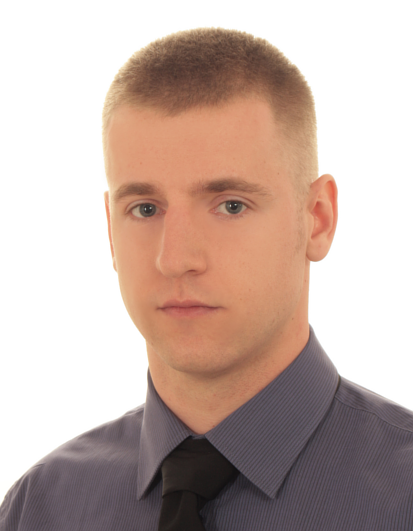
\includegraphics[scale=0.28, right]{photo.png}
        \end{minipage}
        \hspace{0.2cm}
        \begin{minipage}[b]{7cm}
            {\Large \sc Marcin Rainka}
            \begin{description} \itemsep1pt \parskip0pt \parsep0pt
                \item[Adres] ul. PCK 7/80, 81-621 Gdynia
                \item[Data urodzenia] 1 grudzień 1989
                \item[Telefon] (+48) 505 464 392
                \item[E-mail] \href{mailto:marcinrainka@gmail.com}{marcinrainka@gmail.com}
                \item[LinkedIn] \href{https://linkedin.com/in/marcinrainka}{https://linkedin.com/in/marcinrainka}
            \end{description}
        \end{minipage}
    \end{center}

    \vspace{-0.4cm}

    \noindent\rule{\textwidth}{0.1mm}
  
    %==================== PROFIL I CEL ============================================================
  
    \bigskip

    \noindent{\large \bf Profil i cel}
  
    \smallskip

    \noindent
    Pracujący w~niewielkim zespole programista, zaznajomiony z~wieloma technologiami, pragnący poszerzyć swoją~wiedzę oraz~stawić czoła nowym wyzwaniom.
  
    %==================== DOŚWIADCZENIE ZAWODOWE ===================================================

    \bigskip

    \noindent{\large \bf Doświadczenie zawodowe}

    \smallskip

    \noindent{\bf AIC S.A. -- Programista \hfill kwiecień 2014 -- do chwili obecnej}
    \vspace{-0.2cm}
    \begin{itemize} \itemsep1pt \parskip0pt \parsep0pt
        \item Tworzenie aplikacji mobilnych na~platformę~iOS
        \item Rozwój projektu~iProd, śledzącego oraz~kontrolującego pracę automatycznej linii produkcyjnej\linebreak poprzez~iPady
        \item Tworzenie aplikacji desktopowych (WPF)
        \item Tworzenie RESTowych API w technologii Python
        \item Tworzenie aplikacji webowych w oparciu o AngularJS
        \item Pisanie testów automatycznych
        \item Przygotowywanie dokumentacji
    \end{itemize}

    %==================== EDUKACJA =================================================================

    \medskip
  
    \noindent{\large \bf Edukacja}
  
    \smallskip

    \noindent{{\bf Uniwersytet Gdański}, Wydział Matematyki, Fizyki i Informatyki \hfill {\bf 2012 -- 2014}}
    \vspace{-0.2cm}
    \begin{itemize} \itemsep1pt \parskip0pt \parsep0pt
        \item[ ] Studia magisterskie na kierunku Informatyka (tryb dzienny)
    \end{itemize}
    \vspace{-0.2cm}
    \noindent{{\bf Uniwersytet Warmińsko-Mazurski w Olsztynie}, Wydział Matematyki i Informatyki \hfill {\bf2008 -- 2012}}
    \vspace{-0.2cm}
    \begin{itemize} \itemsep1pt \parskip0pt \parsep0pt
        \item[ ] Studia inżynierskie na kierunku Informatyka (tryb dzienny)
    \end{itemize}
    \vspace{-0.2cm}
    \noindent{\bf Liceum Ogólnokształcące nr 1 w Mrągowie \hfill 2005 -- 2008}
    \vspace{-0.2cm}
    \begin{itemize} \itemsep1pt \parskip0pt \parsep0pt
        \item[ ] Matematyka, Fizyka, Informatyka
    \end{itemize}

    %==================== KURSY ====================================================================

    \medskip

    \noindent{\large \bf Dodatkowe kwalifikacje}

    \smallskip

    \noindent{Testowanie automatyczne | Bottega IT Solutions \hfill {\bf kwiecień 2015}}

    \noindent{Craftsmanship, wzorce i architektura dla programistów iOS | Bottega IT Solutions \hfill {\bf październik 2014}}
  
    %==================== UMIEJĘTNOŚCI TECHNICZNE ==================================================

    \bigskip

    \noindent{\large \bf Umiejętności techniczne}
  
    %---------- Języki programowania/znaczników ----------------------------------------------------
  
    \smallskip

    \noindent{\bf Języki programowania/znaczników}

    \smallskip
    $\bullet$ {\bf C\texttt{\#}}
    \hspace{0.34cm}
    $\bullet$ {\bf C\texttt{++}}
    \hspace{0.34cm}
    $\circ$ HTML i CSS
    \hspace{0.34cm}
    $\circ$ JavaScript
    \hspace{0.34cm}
    $\bullet$ {\bf Objective-C}
    \hspace{0.34cm}
    $\bullet$ {\bf Python}
    \hspace{0.34cm}
    $\circ$ Swift
    \hspace{0.34cm}
    $\circ$ TeX

    %---------- Programy graficzne -----------------------------------------------------------------

    \smallskip

    \noindent{\bf Programy graficzne}

    \smallskip
    $\circ$ Blender
    \hspace{0.34cm}
    $\bullet$ {\bf Gimp}
    \hspace{0.34cm}
    $\bullet$ {\bf Inkscape}

    %---------- Pozostałe --------------------------------------------------------------------------

    \smallskip

    \noindent{\bf Pozostałe}

    \smallskip
    $\circ$ AngularJS
    \hspace{0.34cm}
    $\circ$ CUDA
    \hspace{0.34cm}
    $\bullet$ {\bf Flask}
    \hspace{0.34cm}
    $\bullet$ {\bf Git}
    \hspace{0.34cm}
    $\circ$ Jenkins
    \hspace{0.34cm}
    $\circ$ MySQL i MS SQL

    \vspace{0.04cm}
    $\circ$ Redmine
    \hspace{0.34cm}
    $\circ$ SDL
    \hspace{0.34cm}
    $\circ$ Scrum
    \hspace{0.34cm}
    $\bullet$ {\bf Testowanie automatyczne}
    \hspace{0.34cm}
    $\bullet$ {\bf WPF}
  
    %==================== ZAINTERESOWANIA I HOBBY ==================================================

    \bigskip
  
    \noindent{\large \bf Zainteresowania i hobby}
  
    \smallskip
    $\bullet$ Grafika komputerowa
    \hspace{0.34cm}
    $\bullet$ Rysunek i malarstwo
    \hspace{0.34cm}
    $\bullet$ Tworzenie gier komputerowych
    \hspace{0.34cm}
    $\bullet$ Trójbój siłowy
  
    %==================== INNE ====================================================================

    \bigskip
  
    \noindent{\large \bf Inne}
  
    \smallskip
    $\bullet$ Język angielski na poziomie B2 (średnio-zaawansowany)
    \hspace{0.34cm}
    $\bullet$ Prawo jazdy kategorii B
  
    %==================== KLAUZULA =================================================================

    \vspace{1cm}
  
    \noindent \textit{,,Wyrażam zgodę na przetwarzanie moich danych osobowych dla potrzeb
    niezbędnych do realizacji procesu rekrutacji (zgodnie z Ustawą z dnia 29.08.1997 roku o Ochronie
    Danych Osobowych; tekst jednolity: Dz. U. z 2002r. Nr 101, poz. 926 ze zm.).''}
\end{document}
